\documentclass[10pt]{article}
\usepackage{graphicx}
\usepackage{float}
\usepackage{amsmath}
\usepackage{amssymb}
\usepackage{geometry}
\usepackage[utf8]{inputenc}
\usepackage{enumitem}
\usepackage{hyperref}

\geometry{a4paper, top=12mm, left=12mm, right=12mm, bottom=12mm}

% Title information
\title{\Large MESI Cache Coherence Protocol Implementation}
\author{Arinjay Singhal \quad Vihaan Luhariwala}
\date{\today}

\begin{document}

\maketitle

\vspace{-0.5cm}
\begin{center}
\href{https://github.com/BluePanther928/COL216_A3}{GitHub Repository}
\end{center}

\begin{abstract}
\small
This document details the implementation of a cache coherence simulator using the MESI protocol. The simulator models multiple processor cores with private L1 caches communicating over a shared bus, implementing coherence protocols to maintain data consistency across the system.
\end{abstract}

\tableofcontents

\clearpage

% Implementation section
\section{Implementation}
\subsection{Core Classes and Their Structures}
\subsubsection{Cache Class}
\small
The Cache class implements the L1 data cache with:
\begin{itemize}
    \item \textbf{Cache configuration:} Configurable parameters for sets, ways, and block size to support different cache architectures and optimization strategies
    \item \textbf{2D vector structure:} Efficient organization of cache data using a two-dimensional vector, enabling O(1) access time for cache operations
    \item \textbf{LRU counters:} Implementation of Least Recently Used replacement policy to optimize cache utilization and hit rates
    \item \textbf{Statistics tracking:} Comprehensive monitoring of cache performance metrics including hits, misses, and writebacks
\end{itemize}

\subsubsection{CacheLine Structure}
Each cache line maintains:
\begin{itemize}
    \item \textbf{MESI state and dirty bits:} Current coherence state (Modified, Exclusive, Shared, Invalid) and write-back status tracking
    \item \textbf{Tag bits:} Address identification for cache line matching and validation
    \item \textbf{Data block storage:} Actual cached memory content with configurable block size
    \item \textbf{LRU counter:} Dynamic tracking of access patterns for replacement decisions
\end{itemize}

\subsubsection{Bus Class}
The Bus class manages:
\begin{itemize}
    \item \textbf{Bus configuration:} Settings for bus width, transaction types, and connected cores
    \item \textbf{Bus state tracking:} Real-time monitoring of bus availability and current transaction status
    \item \textbf{Transaction management:} Handling of read, write, and coherence messages between caches
    \item \textbf{Coherence statistics:} Collection of bus utilization and protocol overhead metrics
\end{itemize}

\section{Data Structures and Assumptions}
\subsection{Core Data Structures}
\subsubsection{Cache Line Structure}
\begin{itemize}
    \item \textbf{tag:} Address tag bits for cache line identification and matching operations
    \item \textbf{state:} Current MESI protocol state indicating line validity and sharing status
    \item \textbf{data:} Actual memory content stored in the cache line
    \item \textbf{lru\_counter:} Timestamp-based counter for replacement policy implementation
\end{itemize}

\subsubsection{Bus Transaction Structure}
\begin{itemize}
    \item \textbf{type:} Transaction classification (Process/Broadcast) determining handling protocol
    \item \textbf{address:} Target memory address for the current operation
    \item \textbf{requesting\_core:} Identifier of the core initiating the transaction
    \item \textbf{owning\_core:} Identifier of the core currently holding the data
    \item \textbf{data:} Memory content being transferred across the bus
\end{itemize}

\newpage

\subsection{Key Assumptions}
\begin{enumerate}[label=\textbf{\arabic*.}]
    \item Execution cycles: A cycle is counted as execution cycle of a core in following cases:
    \begin{itemize}
        \item Any hit operation is performed which does not require the bus.
        \item Bus is involved in executing the operations due to the corresponding core's instruction.
    \end{itemize}
    \item Idle cycles: A cycle is counted as idle cycle of a core if the core wants to access the bus but it is involved in any other core's operation.
    \item If multiple cores want to access the bus at the same time, then the bus is assigned to the core with the lowest id.
    \item Memory writeback happens in following cases:
    \begin{itemize}
        \item Eviction of Modified lines: due to capacity constrains, the cache line is evicted and written back to the memory. This is counted in execution cycles of the core that caused the eviction.
        \item Bus request of Modified lines: When a cache line is in modified state and other core requests the data, then the data is written back to the memory and this is counted in execution cycles of the core that caused the writeback. The core which writes back to memory is not halted in this case unless it requires the bus (simple read hits can occur in this case).
    \end{itemize}
    \item Reading/Writing from memory takes 100 cycles. So if a single read operation is performed, it takes 100 cycles to complete and an additional cycle to do the read hit. So total 101 cycles.
    \item Cache to Cache data transfer takes 2N cycles where N is the number of words in the cache line. The bus is busy in this case. These cycles are counted in execution cycles of the core that caused the data transfer. The core that supplies the data is not stalled (and can process read hits), if it requests bus access then only it is stalled.
    \item Snooping and initiating bus transaction happens in the same cycle as the miss is detected. Bus is busy until the transaction is completed.
    \item The bus can handle only one transaction at a time. So Snooping signals cannot pass through the bus if it is busy.
    \item Bus transaction signals :
    \begin{itemize}
        \item BusRd: A core requests the bus for read operation.
        \item BusRdX: Read with intent to Modify, this is used when the core wants to read the data and then write to it.
        \item BusUpgr: If the core has a value in Shared state, and it wants to write over it, then it sends BusUpgr signal.
    \end{itemize}
    \item Invalidation counts: Total number of instructions passed by a core which cause invalidation of any cache line in any other core.
    \item If a instruction encounters a cache miss, the miss count is incremented. The miss is counted only once per instruction.
    
    
\end{enumerate}

\section{Function Flowcharts}
\subsection{Main Program Flow}
\begin{figure}[H]
    \centering
    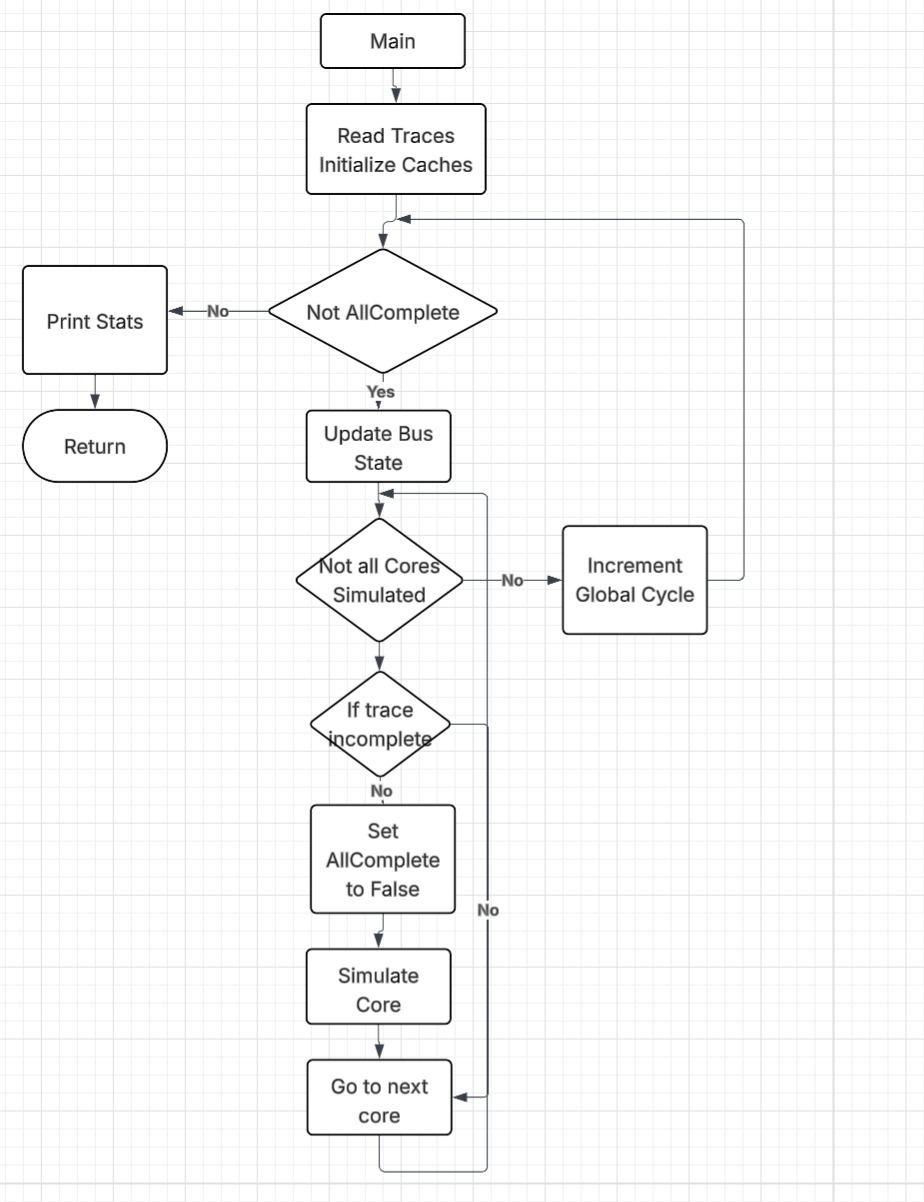
\includegraphics[width=0.75\textwidth]{./images/mainflow.jpg}
    \caption{Main program execution flow}
\end{figure}

\subsection{Bus Transaction Processing}
\begin{figure}[H]
    \centering
    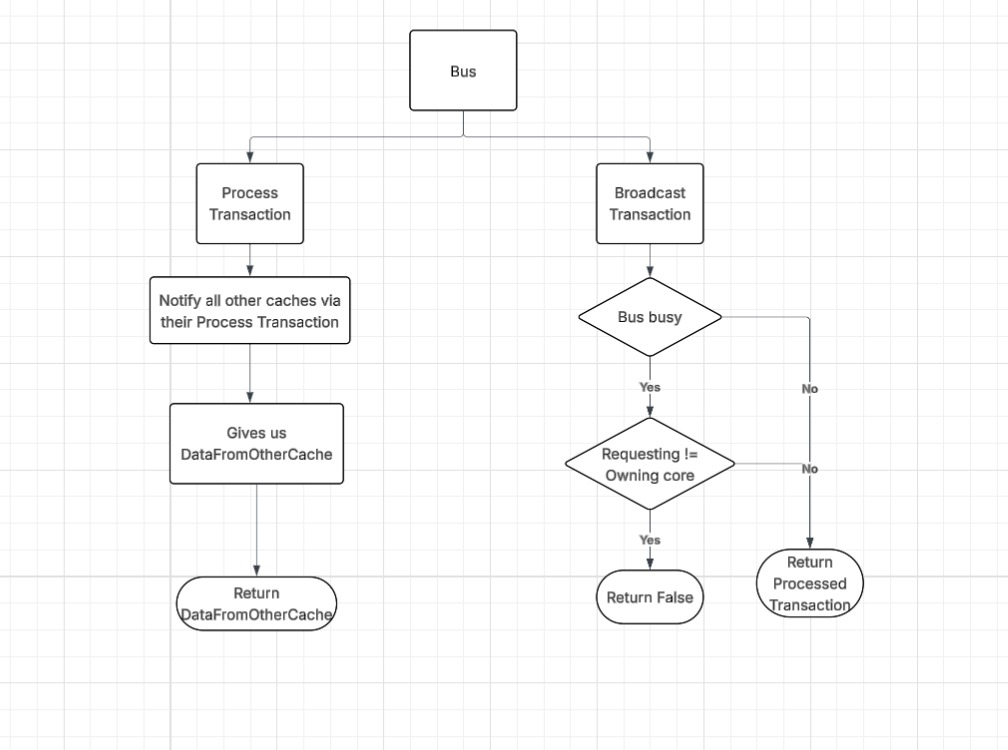
\includegraphics[width=0.75\textwidth]{./images/busflow.jpg}
    \caption{Bus transaction processing flow}
\end{figure}

\subsection{Cache Operations}
\begin{figure}[H]
    \centering
    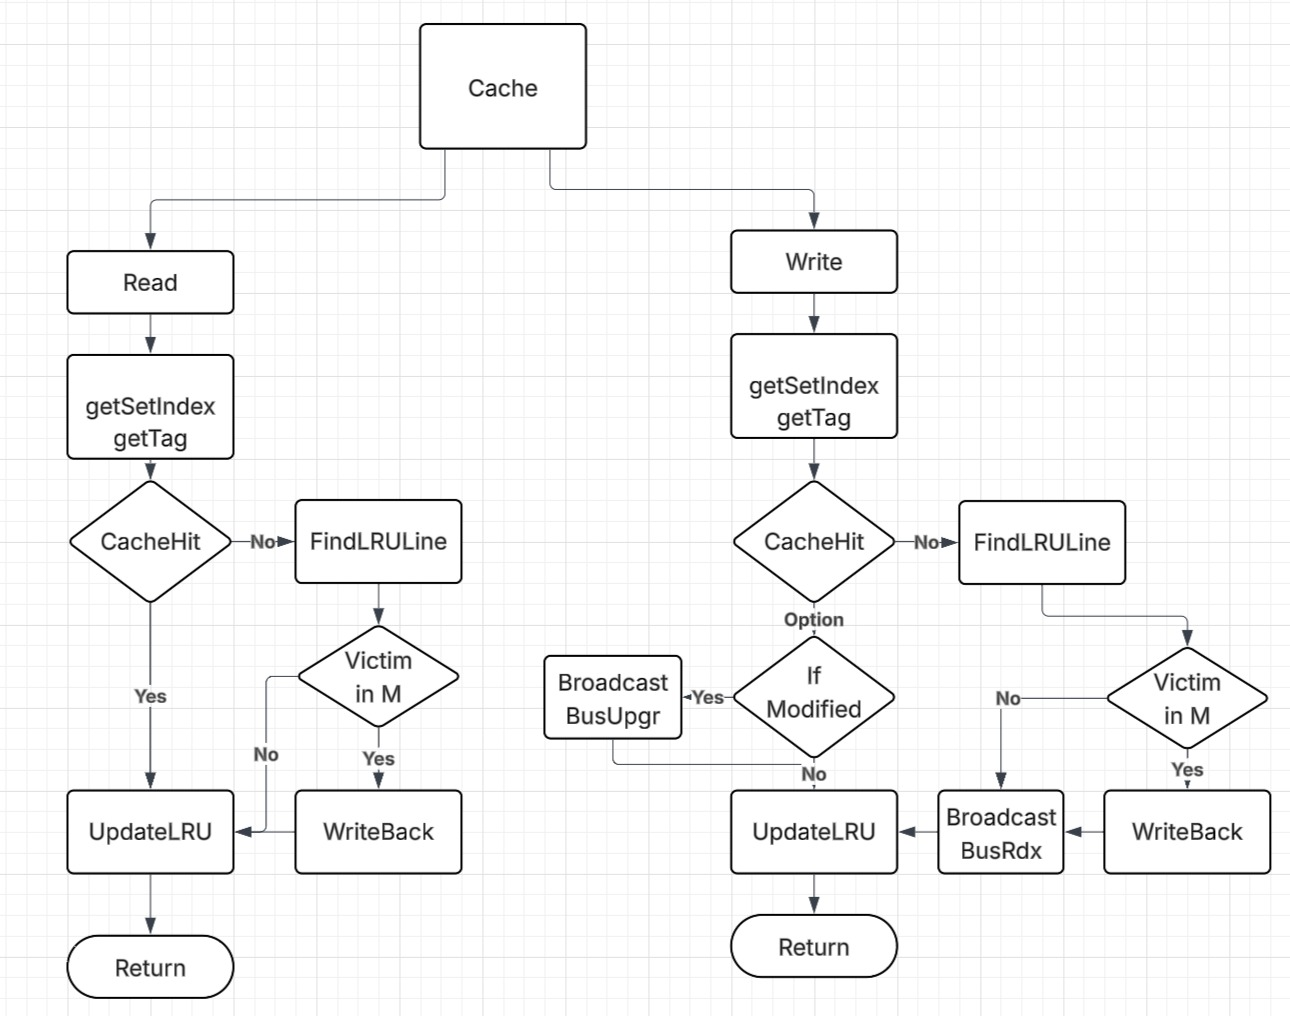
\includegraphics[width=0.75\textwidth]{./Images/cacheflow.jpg}
    \caption{Cache read and write operations}
\end{figure}

\subsection{Process Bus Transaction}
\begin{figure}[H]
    \centering
    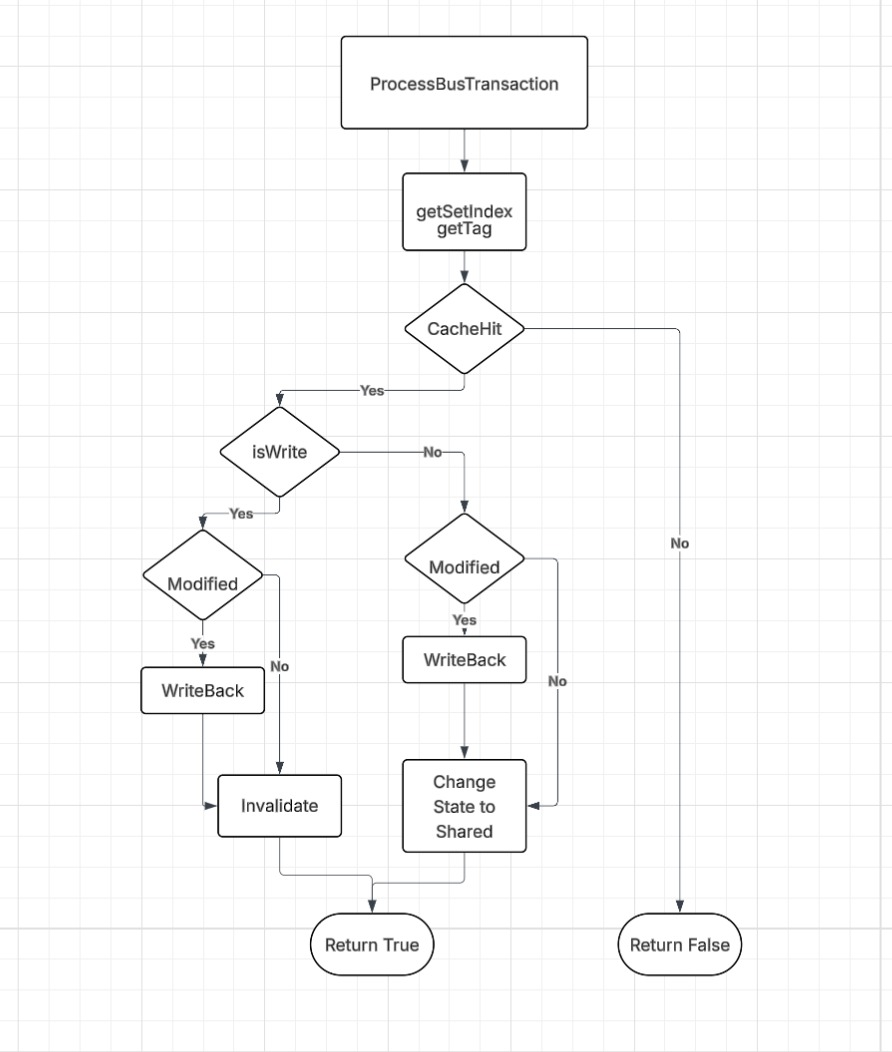
\includegraphics[width=0.75\textwidth]{./Images/bustransactionflow.jpg}
    \caption{Process bus transaction flow}
\end{figure}

\newpage

\section{Protocol Implementation}
\subsection{MESI State Transitions}
The MESI protocol implements state transitions based on bus transactions and local operations:
\begin{itemize}
    \item \textbf{Modified → Shared/Invalid:} Occurs when other cores request read access or line eviction
    \item \textbf{Exclusive → Modified/Shared/Invalid:} Transitions on write hits, read requests, or evictions
    \item \textbf{Shared → Modified/Invalid:} Changes on write operations or invalidation requests
    \item \textbf{Invalid → Modified/Exclusive/Shared:} Results from read/write misses with varying sharing states
\end{itemize}

\section{Performance Evaluation}
\subsection{Benchmark Results}
Performance metrics include:
\begin{itemize}
    \item \textbf{Cache hit/miss rates:} Measurement of cache efficiency and access pattern optimization
    \item \textbf{Bus utilization:} Analysis of bus bandwidth usage and transaction patterns
    \item \textbf{Coherence overhead:} Impact of coherence protocol on system performance
    \item \textbf{Memory access patterns:} Study of spatial and temporal locality in applications
\end{itemize}

\section{Trace Analysis}
Note: We have implemented LRU policy in case of bus access races. This makes our model deterministic. So the rubric where we have to generate multiple runs for same parameters are not applicable to us.
\subsection{False Sharing Analysis}
False sharing occurs when multiple processors access different data items that happen to be stored in the same cache line. This analysis compares the performance impact of false sharing with different block sizes. Traces are available in falsesharing folder.

\subsubsection{Block Size = 5 (32 bytes)}
\begin{itemize}
    \item Cache Miss Rate: 66.67\% across all cores
    \item Execution Cycles:
    \begin{itemize}
        \item Core 0: 303 cycles
        \item Core 1: 403 cycles
        \item Core 2: 403 cycles
        \item Core 3: 403 cycles
    \end{itemize}
    \item Idle Cycles:
    \begin{itemize}
        \item Core 0: 199 cycles
        \item Core 1: 300 cycles
        \item Core 2: 899 cycles
        \item Core 3: 1100 cycles
    \end{itemize}
\end{itemize}

\subsubsection{Block Size = 2 (4 bytes)}
\begin{itemize}
    \item Cache Miss Rate: 33.33\% across all cores
    \item Execution Cycles:
    \begin{itemize}
        \item Core 0: 103 cycles
        \item Core 1: 103 cycles
        \item Core 2: 103 cycles
        \item Core 3: 103 cycles
    \end{itemize}
    \item Idle Cycles:
    \begin{itemize}
        \item Core 0: 0 cycles
        \item Core 1: 100 cycles
        \item Core 2: 200 cycles
        \item Core 3: 300 cycles
    \end{itemize}
\end{itemize}

\subsubsection{Analysis of False Sharing}
The results demonstrate the impact of false sharing on system performance:
\begin{itemize}
    \item \textbf{High Miss Rates:} The 66.67\% miss rate indicates frequent cache line invalidations due to false sharing
    \item \textbf{Bus Contention:} All bus transactions are BusRdX, showing that writes are causing coherence traffic
    \item \textbf{Performance Impact:} The high number of writebacks and invalidations indicates significant overhead from false sharing
    \item \textbf{Block Size Effect:} Larger block sizes (b=5) exacerbate false sharing as more data items share the same cache line
\end{itemize}

\subsection{LRU testing}

The test case has the following parameters:
\begin{itemize}
    \item Set Index Bits (s) = 0
    \item Associativity (E) = 3
    \item Block Size (b) = 2 (4 bytes)
\end{itemize}

This configuration results in a single set with 3 possible ways. The test sequence demonstrates the LRU replacement policy:

\begin{enumerate}
    \item Initial compulsory read misses for addresses 0x0, 0x4, and 0x8 establish the initial LRU order: 0x0, 0x4, 0x8
    \item A subsequent read to 0x4 updates the LRU order to: 0x0, 0x8, 0x4
    \item Two write operations to 0xC and 0x10 trigger evictions:
    \begin{itemize}
        \item First write to 0xC evicts 0x0, resulting in LRU order: 0x8, 0x4, 0xC
        \item Second write to 0x10 evicts 0x8, completing the sequence
    \end{itemize}
\end{enumerate}

This behavior was verified through debug mode execution, confirming the correct LRU order and eviction sequence.

\subsubsection{Data Traffic Analysis}
\begin{figure}[H]
    \centering
    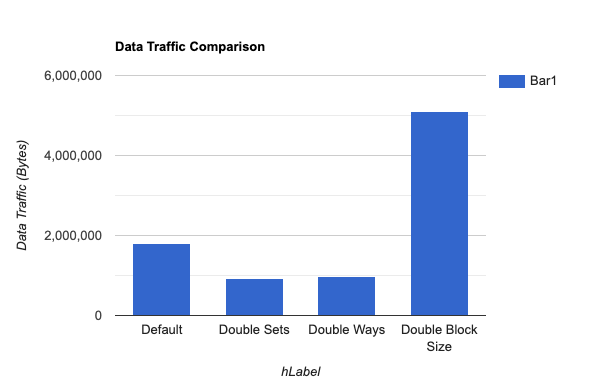
\includegraphics[width=0.8\textwidth]{./images/data_traffic.png}
    \caption{Data Traffic Comparison for Different Cache Configurations}
\end{figure}

The data traffic analysis reveals significant variations across different cache configurations:

\begin{itemize}
    \item \textbf{Block Size Impact:} Doubling block size causes the highest data traffic due to larger memory transfers per miss. While this can potentially improve spatial locality, it significantly increases bandwidth usage.
    
    \item \textbf{Cache Organization:} Doubling sets or ways reduces data traffic, indicating fewer memory accesses and better cache efficiency. This suggests that increasing cache capacity through either more sets or higher associativity can effectively reduce memory bandwidth requirements.
    
    \item \textbf{Trade-offs:} While larger blocks can increase spatial locality by prefetching nearby data, they also lead to increased bandwidth usage. This highlights the importance of balancing spatial locality benefits against bandwidth constraints in cache design.
\end{itemize}

\subsubsection{Evictions Analysis}
\begin{figure}[H]
    \centering
    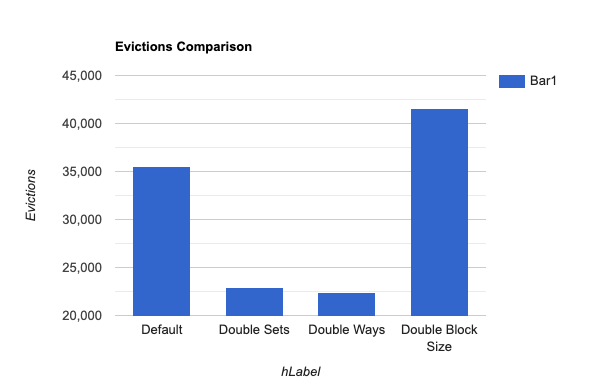
\includegraphics[width=0.8\textwidth]{./images/evictions.png}
    \caption{Cache Evictions Comparison for Different Cache Configurations}
\end{figure}

The evictions analysis demonstrates how different cache parameters affect the frequency of cache line replacements:

\begin{itemize}
    \item \textbf{Cache Capacity Impact:} Double sets and double ways result in the fewest cache evictions, thanks to greater capacity and associativity. This demonstrates how increased cache space reduces conflict and capacity misses.
    
    \item \textbf{Block Size Effect:} Double block size leads to the most evictions, as fewer larger blocks fit in the cache. This illustrates the trade-off between block size and effective cache utilization.
    
    \item \textbf{Baseline Performance:} The default configuration shows moderate evictions, reflecting limited cache flexibility. This serves as a reference point for evaluating optimization strategies.
\end{itemize}

\subsubsection{Execution Cycles Analysis}
\begin{figure}[H]
    \centering
    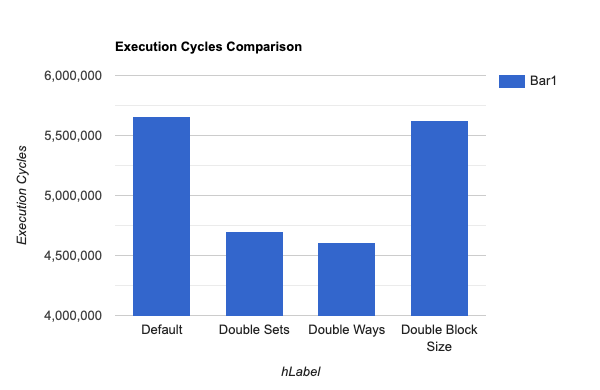
\includegraphics[width=0.8\textwidth]{./images/exec_cycles.png}
    \caption{Execution Cycles Comparison for Different Cache Configurations}
\end{figure}

The execution cycles analysis reveals the impact of cache configurations on overall performance:

\begin{itemize}
    \item \textbf{Associativity Impact:} Doubling the number of ways yields the lowest execution cycles, improving performance. This suggests that increased associativity effectively reduces conflict misses and improves cache utilization.
    
    \item \textbf{Set Size Effect:} Double sets also improve performance, but slightly less than double ways. This indicates that while increasing the number of sets reduces conflicts, the benefit is not as pronounced as increasing associativity.
    
    \item \textbf{Block Size Trade-off:} Double block size performs similarly to default, suggesting performance gains from spatial locality are offset by higher miss costs. This demonstrates the complex balance between exploiting spatial locality and managing cache space efficiently.
\end{itemize}

\subsubsection{Idle Cycles Analysis}
\begin{figure}[H]
    \centering
    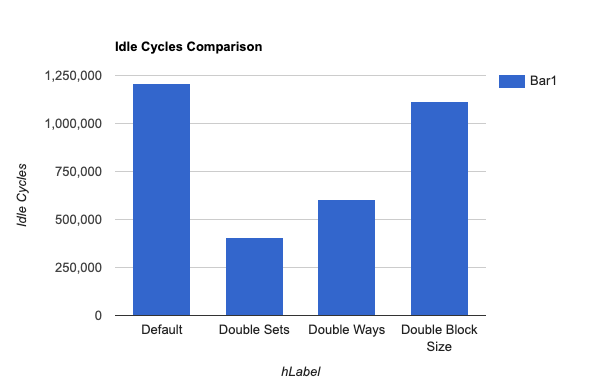
\includegraphics[width=0.8\textwidth]{./images/idle_cycles.png}
    \caption{Idle Cycles Comparison for Different Cache Configurations}
\end{figure}

The idle cycles analysis provides insights into memory-related stalls across different configurations:

\begin{itemize}
    \item \textbf{Set Size Efficiency:} Double sets show the least idle time, indicating fewer memory stalls. This suggests that increasing the number of sets leads to better distribution of cache lines and reduced contention for memory access.
    
    \item \textbf{Associativity Benefits:} Double ways also reduce idle cycles, due to better hit rates. The increased associativity helps avoid conflict misses, resulting in fewer memory access delays.
    
    \item \textbf{Block Size Impact:} Double block size increases idle time, as larger misses take longer to fetch. This highlights how larger block sizes can lead to increased memory access latency despite potential spatial locality benefits.
    
    \item \textbf{Default Limitations:} The default configuration shows the most idle cycles, indicating frequent memory-related stalls. This baseline performance suggests significant room for improvement through cache parameter optimization.
\end{itemize}

\subsubsection{Invalidations Analysis}
\begin{figure}[H]
    \centering
    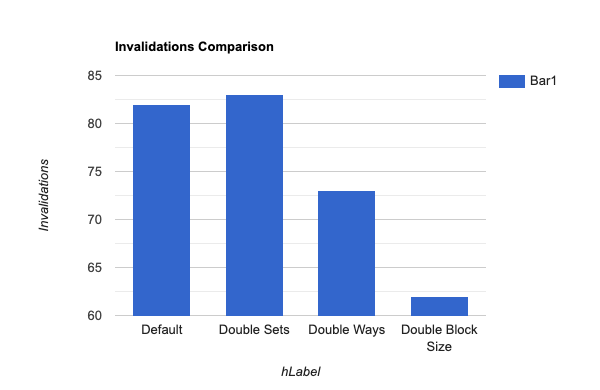
\includegraphics[width=0.8\textwidth]{./images/invalidations.png}
    \caption{Cache Invalidations Comparison for Different Cache Configurations}
\end{figure}

The invalidations analysis reveals the coherence behavior in the multicore environment:

\begin{itemize}
    \item \textbf{Block Size Effect:} Double block size results in the fewest invalidations, possibly due to fewer, larger blocks being shared. This suggests that larger blocks may reduce coherence traffic in certain workloads, despite their other performance trade-offs.
    
    \item \textbf{Set Size Impact:} Double sets lead to the most invalidations, likely due to more active cache blocks in a multicore environment. While more sets improve overall cache utilization, they may increase coherence overhead in shared memory scenarios.
    
    \item \textbf{Associativity Influence:} Double ways shows moderate improvement in invalidations compared to the default, suggesting that increased associativity can help manage coherence traffic while maintaining good cache utilization.
\end{itemize}

\subsubsection{Miss Rate Analysis}
\begin{figure}[H]
    \centering
    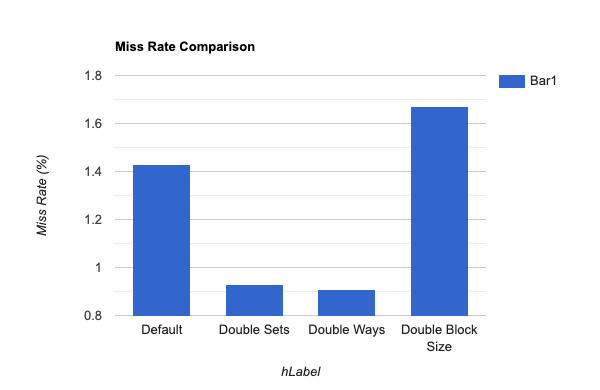
\includegraphics[width=0.8\textwidth]{./images/miss_rate.png}
    \caption{Cache Miss Rate Comparison for Different Cache Configurations}
\end{figure}

The miss rate analysis demonstrates the effectiveness of different cache organizations:

\begin{itemize}
    \item \textbf{Cache Organization Benefits:} Double sets and double ways significantly reduce miss rate, improving cache hit efficiency. This demonstrates how both increased associativity and more sets can effectively reduce conflict misses and improve overall cache performance.
    
    \item \textbf{Block Size Impact:} Double block size increases miss rate, as fewer blocks reduce flexibility and increase conflict/capacity misses. This higher miss rate suggests that the potential benefits of spatial locality are outweighed by the reduced number of cache blocks available.
    
    \item \textbf{Baseline Performance:} Default configuration has a moderate miss rate, with room for improvement. This indicates that simple modifications to cache parameters can yield significant performance benefits.
\end{itemize}

\subsubsection{Total Program Cycles Analysis}
\begin{figure}[H]
    \centering
    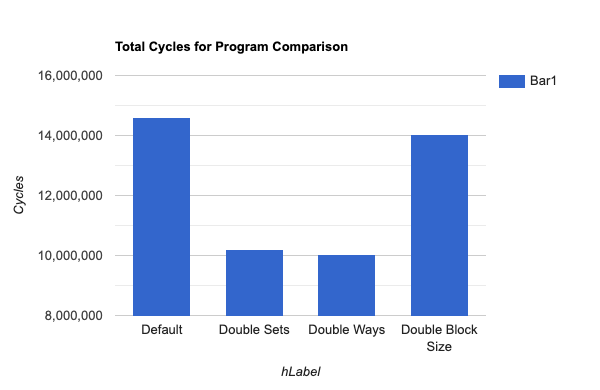
\includegraphics[width=0.8\textwidth]{./images/total_cycles.png}
    \caption{Total Program Cycles Comparison for Different Cache Configurations}
\end{figure}

The total program cycles analysis provides a comprehensive view of overall system performance:

\begin{itemize}
    \item \textbf{Set Size Impact:} Double Sets reduce total cycles by about 30\% (from 14.5M to 10.2M), offering a significant performance boost through reduced conflict misses. This substantial improvement demonstrates the effectiveness of increasing cache capacity through additional sets.
    
    \item \textbf{Associativity Benefits:} Double Ways perform slightly better than double sets (10M cycles), benefiting from higher associativity that improves cache efficiency. This suggests that increased associativity is particularly effective at reducing conflict misses in this workload.
    
    \item \textbf{Block Size Effect:} Double Block Size shows minimal improvement (14M cycles), suggesting limited benefit from larger blocks due to poor spatial locality in the workload. This indicates that simply increasing block size may not be effective without considering the application's memory access patterns.
    
    \item \textbf{Default Limitations:} Default configuration has the highest total cycles (14.5M), reflecting inefficient cache behavior and frequent memory stalls. This baseline performance emphasizes the potential for significant improvements through cache parameter optimization.
\end{itemize}

\subsubsection{Write Backs Analysis}
\begin{figure}[H]
    \centering
    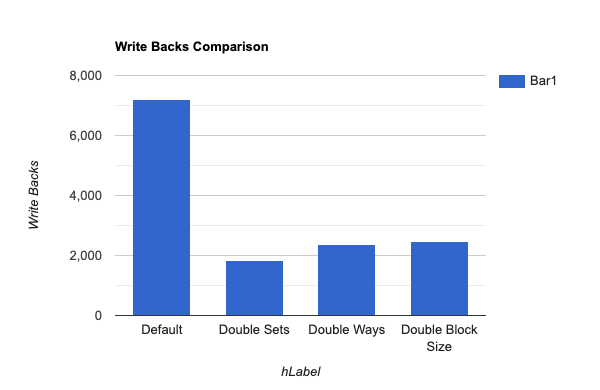
\includegraphics[width=0.8\textwidth]{./images/write_backs.png}
    \caption{Write Backs Comparison for Different Cache Configurations}
\end{figure}

The write backs analysis reveals how different cache configurations affect memory write traffic:

\begin{itemize}
    \item \textbf{Set Size Efficiency:} Double Sets reduce write backs drastically (from 7,300 to 1,800), showing the best performance by minimizing evictions of dirty blocks. This significant reduction demonstrates how increased set count can effectively reduce capacity-related writebacks.
    
    \item \textbf{Associativity Impact:} Double Ways achieve a 67\% reduction (to 2,400 write backs), effectively lowering write-backs through improved associativity, but not as efficiently as doubling sets. This suggests that while higher associativity helps, set organization has a more significant impact on write-back behavior.
    
    \item \textbf{Block Size Effect:} Double Block Size results in 2,500 write backs, slightly higher than double ways, as larger blocks group writes better but don't reduce eviction pressure as much. This shows the trade-off between spatial write grouping and cache space utilization.
    
    \item \textbf{Default Limitations:} Default configuration has the highest write backs (7,300), caused by frequent eviction of modified lines in a limited cache space. This indicates significant room for improvement in write-back efficiency through cache parameter optimization.
\end{itemize}




\section{Conclusion}
The implementation demonstrates a functional MESI cache coherence protocol with:
\begin{itemize}
    \item \textbf{Efficient state management:} Optimized handling of cache line states and transitions
    \item \textbf{Proper coherence maintenance:} Reliable data consistency across multiple caches
    \item \textbf{Scalable multi-core support:} Architecture supporting varying numbers of cores
    \item \textbf{Reliable performance metrics:} Comprehensive monitoring and analysis capabilities
\end{itemize}


\end{document}
